\section{Estimators}
\label{sec:estimators}

\subsection{Bias and Variance}
\label{sec:BandV}

First let us recall the standard definitions of {\em Bias}\ and {\em Variance}.
Following the approach in Ref.~\cite{Mehta:2018dln}, we consider a set of $n$
data points, which we denote $D_n=\left(x,y\right)$, where $x,y \in \Rn$,
generated according to some noisy model:
\begin{equation}
    \label{eq:NoisyData}
    y_i = f(x_i) + \epsilon_i\, ,
\end{equation}
where $\epsilon\sim\mathcal{N}(0,\sigma)$. The function $g(x,\theta)$, which
depends on a set of parameters $\theta$, allows us to predict the value of $y$
for a new data point $x_{n+1}$. It is obtained by minimizing some cost function,
\eg
\begin{equation}
    \label{eq:CostFuncChi}
    \chi^2(\theta; D_n) = \sum_{i=1}^n
    \frac{\Big(
        y_i - g(x_i,\theta)
    \Big)^2}{\sigma_i^2}\, .
\end{equation}
Note that whilst here we are considering the case of a diagonal covariance matrix.
All of the arguments hold when there are correlations, since we can easily just
consider everything in the basis which diagonalises the covariance matrix. The
best fit for a given set of data is
\begin{equation}
    \label{eq:ThetaMin}
    \theta_D = {\arg\min}_\theta \chi^2(\theta; D_n)\, .
\end{equation}

%Clearly the value of $\chi^2$ at the minimum depends on the particular dataset
%\begin{equation}
%    \label{eq:ChiAtMin}
%    \chi^2_\mathrm{min}=\chi^2(\theta_D; D_n)\, .
%\end{equation}
%We will be drawing an ensemble of datasets from the distribution above,
%and denote by $\mathbb{E}_D$ the average over these datasets.
Clearly the parameters which minimise $\chi^2$ for a given set of data points
depends on $D_n$, denoted by the subscript $D$. In the end we are interested in
defining a generalization error on a finite set of total data which we split
into two subsets, data used in the training procedure
(both training and validation) which we denote as $\{ D \}$
and data used as a test set which we define as $\{ D' \}$. The generalization
error is then defined as
\begin{equation}
    \label{eq:DefGenErr}
    \chi^2(\theta_D; D'_{n'}) = \sum_{i=1}^{n'}
    \frac{\Big(
        y'_i - g(x'_i,\theta_D)
    \Big)^2}{\sigma_i^2}\, ,
\end{equation}
where we have very explicitly defined that the generalization error is where we
take the function $g$ with parameters fitted on $D_n$ and then calculate the
$\chi^2$ of this function compared to the test set data $D'_{n'}$.

Replicas of the function $g$ can be fitted on the same set of points $\{ x\}$
but with different ensembles of noise $\{ \epsilon\} $, which is the same as
the Monte-Carlo replicas we use in current fits. We define the average over the
Gaussian variable $\epsilon$ by $\mathbb{E}_\epsilon$. Care should be taken
since both the data $D_n$ and the function $g(x,\theta_D)$ depend on $\epsilon$.
The generalization error can then be decomposed, with the expectation over
$\epsilon$ taken
\begin{align}
    \label{eq:GenErr}
    &\mathbb{E}_{\epsilon}\left[\chi^2(\theta_D; D'_{n'})/n'\right] = \nonumber \\
    &\quad = \mathbb{E}_{\epsilon}\left[
        \frac{1}{n'}\, \sum_{i=1}^{n'}
        \frac{\Big(
            y'_i - g(x'_i,\theta_D)
        \Big)^2}{\sigma_i^2}
    \right] \\
    &\quad = \frac{1}{n'}\, \sum_{i=1}^{n'} \left[
        \frac{\mathbb{E}_\epsilon\left[
            \Big(y'_i - f(x'_i)\Big)^2
        \right]}{\sigma_i^2}
        + \frac{\mathbb{E}_{\epsilon}\left[\Big(f(x'_i)-g(x'_i,\theta_D)\Big)^2\right]}{\sigma_i^2}
    \right] \\
    &\quad = 1 + \frac{1}{n'}\, \sum_{i=1}^{n'} \left[
            \frac{\Big(f(x'_i) - \mathbb{E}_{\epsilon}\left[g(x'_i,\theta_D)\right]\Big)^2}{\sigma_i^2}
        \right] + \nonumber \\
    &\quad \quad +
        \frac{1}{n'}\, \sum_{i=1}^{n'} \left[
            \frac{
                \Ebb_{\epsilon}\left[\Big(g(x'_i,\theta_D) -
                \Ebb_{\epsilon}\left[g(x'_i,\theta_D)\right]\Big)^2\right]
            }{\sigma_i^2}
        \right]\, .
\end{align}
These three contributions are known as {\em Noise}, {\em Bias}\ and {\em Variance}
respectively.

\subsection{Bias and Variance for \nnpdf\ fit}

Whilst it is clear in the \nnpdf\ case the average of $\epsilon$ is the average
over replicas (or level 2 noise), it isn't entirely clear what will happen in
the presence of a level 1 shift $\eta$. Even outside of a closure test it is
understood that the central values given by experimentalists implictly contain
a term like $\eta$ such that we can define $\mathcal{D} = (x, \levone)$ such that
$\levone$ represents the level 1 data or experimental central value
\begin{equation}
    \label{eq:DefLev1}
    \levone_{i} = f(x_i) + \eta_i \, ,
\end{equation}
and then the level 2 data is defined as
\begin{align}
    \label{eq:DefLev2}
    y_{i} &= \levone_i + \epsilon_i \\
    &= f(x_i) + \eta_i  + \epsilon_i \, .
\end{align}
Also at the end of the fit we don't calculate $\chi^2(\theta_D; D_n)$ comparing
the fitted function to the noisey level 2 data but instead calculate something
like
\begin{equation}
    \label{eq:DefRepChi2}
    \chi^2(\theta_D; \mathcal{D}_{n}) = \sum_{i=1}^{n}
    \frac{\Big(
        \levone_i - g(x_i,\theta_D)
    \Big)^2}{\sigma_i^2}\, ,
\end{equation}
the $\chi^2$ of a given replica function on the level 1 data. We can still
consider calculating this object on a test set $\mathcal{D}'_{n'}$ and then
taking the expectation across replicas and perform the decomposition as before
\begin{align}
    & \mathbb{E}_{\epsilon}\left[\chi^2(\theta_D; \mathcal{D}'_{n'})/n'\right] = \nonumber\\
    & \quad = \mathbb{E}_{\epsilon}\left[
        \frac{1}{n'}\, \sum_{i=1}^{n'}
        \frac{\left(
            \levone'_i - g(x'_i,\theta_D)
        \right)^2}{\sigma_i^2}
    \right] \\
    & \quad = \frac{1}{n'}\, \sum_{i=1}^{n'} \Bigg[
        \frac{\left[
            \left(\levone'_i - f(x'_i)\right)^2
        \right]}{\sigma_i^2}
        + \frac{
            \mathbb{E}_{\epsilon}\left[\left(f(x'_i)-g(x'_i,\theta_D)\right)^2\right]
            }{\sigma_i^2} + \nonumber \\
    & \quad \quad + 2\frac{\mathbb{E}_{\epsilon}
    \left[
        \left(\levone'_i - f(x'_i)\right)\left(f(x'_i)-g(x'_i,\theta_D)\right)
    \right]}{\sigma_i^2}
    \Bigg] \\
    & \quad = \frac{1}{n'}\, \sum_{i=1}^{n'}
        \frac{{\eta'}_i^2}{\sigma_i^2} +
    \frac{1}{n'}\, \sum_{i=1}^{n'} \frac{
        \left(f(x'_i) - \mathbb{E}_{\epsilon}\left[g(x'_i,\theta_D)\right]\right)^2
        }{\sigma_i^2} + \nonumber \\
    & \quad \quad +
    \frac{1}{n'}\, \sum_{i=1}^{n'} \frac{
                \Ebb_{\epsilon}\left[\Big(g(x'_i,\theta_D) -
                \Ebb_{\epsilon}\left[g(x'_i,\theta_D)\right]\Big)^2\right]
            }{\sigma_i^2} + \nonumber \\
    & \quad \quad -
    \frac{1}{n'}\, 2 \sum_{i=1}^{n'} \frac{\mathbb{E}_{\epsilon}
        \left[
            \left(\levone'_i - f(x'_i)\right)\left(g(x'_i,\theta_D) - f(x'_i)\right)
        \right]}{\sigma_i^2} \, . \label{eq:NNPDFGenErr}
\end{align}
In \eqref{eq:NNPDFGenErr} we now have 4 terms, the level 1 {\em Noise},
{\em Bias}, {\em Variance} and a cross term respectively.

\paragraph[]{Note:} It's important to note that whilst the $\chi^2$ here was
calculated on level 1 data, the only difference between calculating this quantity
on level 1 vs. level 2 data is the Noise term, which is the least interesting
term since it adds either 1 or 2 to the expectation of $\chi^2$ depending on
whether we are looking at level 1 or level 2 data respectively, up to finite
data fluctuations.

\paragraph[]{}
The cross term can
be thought of as the pull of the level 1 data on the underlying law times by
the pull of the fitted function on the underlying law. Take care with the minus
sign that was brought out the front of the cross term. The expectation over
$\epsilon$ of the \nnpdf\ generalization error is currently called
$\langle \chi^2 \rangle$ in our reports with the key difference being that
$\chi^2$ calculated on some test set of data. At present in a closure
test report by default we have
$\mathbb{E}_{\epsilon}\left[\chi^2(\theta_D; \mathcal{D}_{n})/n'\right]$,
{\em Bias} and {\em Variance}. We also have $\Delta_{\chi^2}$ which will be
dealt with in the next section along with the cross term we see above.

\paragraph[]{Averages:} There is a residual dependence
on the splitting of data into in-sample and test sets, with fast fits one can
actually perform multiple fits on different splits and take compare the above
estimators across different splits.

\subsection{Completing the closure test estimator picture}

In the previous section we spoke about the terms which appear when decomposing
the expectation across replicas of $\chi^2$. We can explicitly define the
closure test estimators in the notation used above dropping the prime notation
which just indicates that the estimator should be calculated on test set data
if it is to be thought of as generalization.

\subsubsection*{Bias}

The bias is defined as the $\chi^2$ between the expected value of the model
across replicas, $g(x, \theta_D)$, and the level 0 data,
$f(x)$. This is clearly a measure of how far away the
central prediciction is away from the underlying law, explictly defined as
%
\begin{equation}
    \label{eq:Biasdef}
    \mathrm{bias} = \frac{1}{n} \sum_{i=1}^{n} \frac{(f(x_i) -
    \Ebb_{\epsilon}\left[g(x_i,\theta_D)\right])^2}{\sigma_i^2} \, .
\end{equation}
%
Since we are aiming to produce the PDF set, the goal of a fit is to reproduce
the underlying law. The caveat is that we can only calculate the bias in a
closure test setting, and clearly don't have access to this quantity in a fit to
experimental data.

Adding parameters to the model
typically lowers the bias as the model has freedom to fit the data better, however at some point the
cost for lowering the bias is that the variance of the model increases. In our
case it's not as clear cut, since we have added a level 1 noise, and so adding
additional parameters to the model could lead to a lower $\chis$ without the bias
actually decreasing.

\subsubsection*{Variance}

This quantity goes alongside the bias and tells us the variability of the
$\chis$ with the model. We already use this estimator in the fits, by a
different name $\varphi$, in the case of a closure defined as
%
\begin{equation}
    \begin{split}
        \mathrm{variance} &= \frac{1}{n}\, \sum_{i=1}^{n} \frac{
            \Ebb_{\epsilon}\left[\Big(g(x_i,\theta_D) -
            \Ebb_{\epsilon}\left[g(x_i,\theta_D)\right]\Big)^2\right]
        }{\sigma_i^2} \, .
    \end{split}
\end{equation}
%
We see
that the variance is just the average spread of replicas in units of the
experimental error.

Generally the aim of fitting is to reduce the bias whilst retaining a reasonable
variance - this is commonly referred to as the bias-variance tradeoff. Again
in the PDF fit there is a slight difference that the variance represents our PDF
error and should be larger than the bias to ensure that the errorband on our
PDF represents a reasonable quantile the true underlying law should reside
within. A high bias low variance PDF would clearly be problematic.

\subsubsection*{Delta chi2}

The final estimator, $\dcs$, doesn't obviously appear in the decomposition of \newline
$\mathbb{E}_{\epsilon}\left[\chi^2(\theta_D; \mathcal{D}_{n})/n'\right]$.
When it was introduced it was said to describe how well the model matched the
underlying law. We start with the definition of the $\dcs$ with the notation
used in this note
%
\begin{equation}
        \dcs = \frac{
            \sum_{i=1}^{n} \frac{(z_i -
            \Ebb_{\epsilon}\left[g(x_i,\theta_D)\right])^2}{\sigma_i^2} -
            \sum_{i=1}^n \frac{\eta_i^2}{\sigma_i^2}}{
                \sum_{i=1}^n \frac{\eta_i^2}{\sigma_i^2}} \, .
\end{equation}
Alongside $\dcs$ there were some bounds:
%
\begin{itemize}
    \item $\dcs < 0$ overfitting
    \item $\dcs = 0$ perfect fit
    \item $\dcs > 0$ underfitting
\end{itemize}
%
which seem intuitive but the discussion of these bounds implies that bias and
$dcs$ are linked, which is not immediately obvious. We can rewrite
$\dcs$ removing the normalization over the noise and replacing with normalization
over number of data points (which in the limit of infinite Gaussian data are
the same)
%
\begin{equation}
    \begin{split}
        \dcs &= \frac{1}{n}\left[ \sum_{i=1}^{n} \frac{(z_i -
        \Ebb_{\epsilon}\left[g(x_i,\theta_D)\right])^2}{\sigma_i^2} -
        \sum_{i=1}^n \frac{\eta_i^2}{\sigma_i^2} \right] \\
        &= \frac{1}{n}\left[ \sum_{i=1}^{n} \frac{(z_i - f(x_i) + f(x_i) -
        \Ebb_{\epsilon}\left[g(x_i,\theta_D)\right])^2}{\sigma_i^2} -
        \sum_{i=1}^n \frac{\eta_i^2}{\sigma_i^2} \right] \\
        &= \frac{1}{n} \left[ \sum_{i=1}^{n} \frac{(f(x_i) -
        \Ebb_{\epsilon}\left[g(x_i,\theta_D)\right])^2}{\sigma_i^2} -
        2\sum_{i=1}^n \frac{
            (z_i - f(x_i))(\Ebb_{\epsilon}\left[g(x_i,\theta_D)\right] - f(x_i))}{
                \sigma_i^2}\right]
    \end{split}
    \label{eq: deltachi2tobias}
\end{equation}
%
we recognise the first term in the numerator as the bias, and the second term
as the cross term which appeared in \eqref{eq:NNPDFGenErr}. This completes
our understanding of closure test estimators and how they link to both
expectation of $\chi^2$ across replicas, Summarising:
%
\begin{align}
    &\mathbb{E}_{\epsilon}\left[\chi^2(\theta_D; \mathcal{D}'_{n'})/n'\right] = \nonumber \\
    & \quad = \mathrm{noise} \, + \, \mathrm{bias} \, + \, \mathrm{variance} \, - \, \mathrm{cross \ term} \\
    & \quad = \mathrm{noise} + \dcs \, + \, \mathrm{variance} \\
    & \quad = \chi^2[\Ebb_{\epsilon}\left[g(x_i,\theta_D)\right], \mathcal{D}_n] + \, \mathrm{variance}
\end{align}
%
We now see that $\dcs < 0$
corresponds to expected value of model,
$\mathbb{E}_{\epsilon}\left[\chi^2(\theta_D; \mathcal{D}'_{n'})/n'\right]$
moving away from the level 0 data specifically in the direction of the level 1
data. $\dcs = 0$ does not necessarily refer to the model perfectly reproducing the underlying law,
although clearly this is one case which would lead to $\dcs=0$.
Finally $\dcs > 0$ refers to the theory prediction moving
away from the underlying law but not towards the level 1 data, which suggests a
poor fit.

These new definitions are not in conflict with the original bounds above but
offer a bit more insight into the subtle cases where both the bias can increase,
but $\dcs$ becomes closer to zero.

We can visualise the above with a simple example in 2D, shown in figure
\ref{fig:vectorexample}
\newpage
%
\begin{figure}[!h]
    \centering
    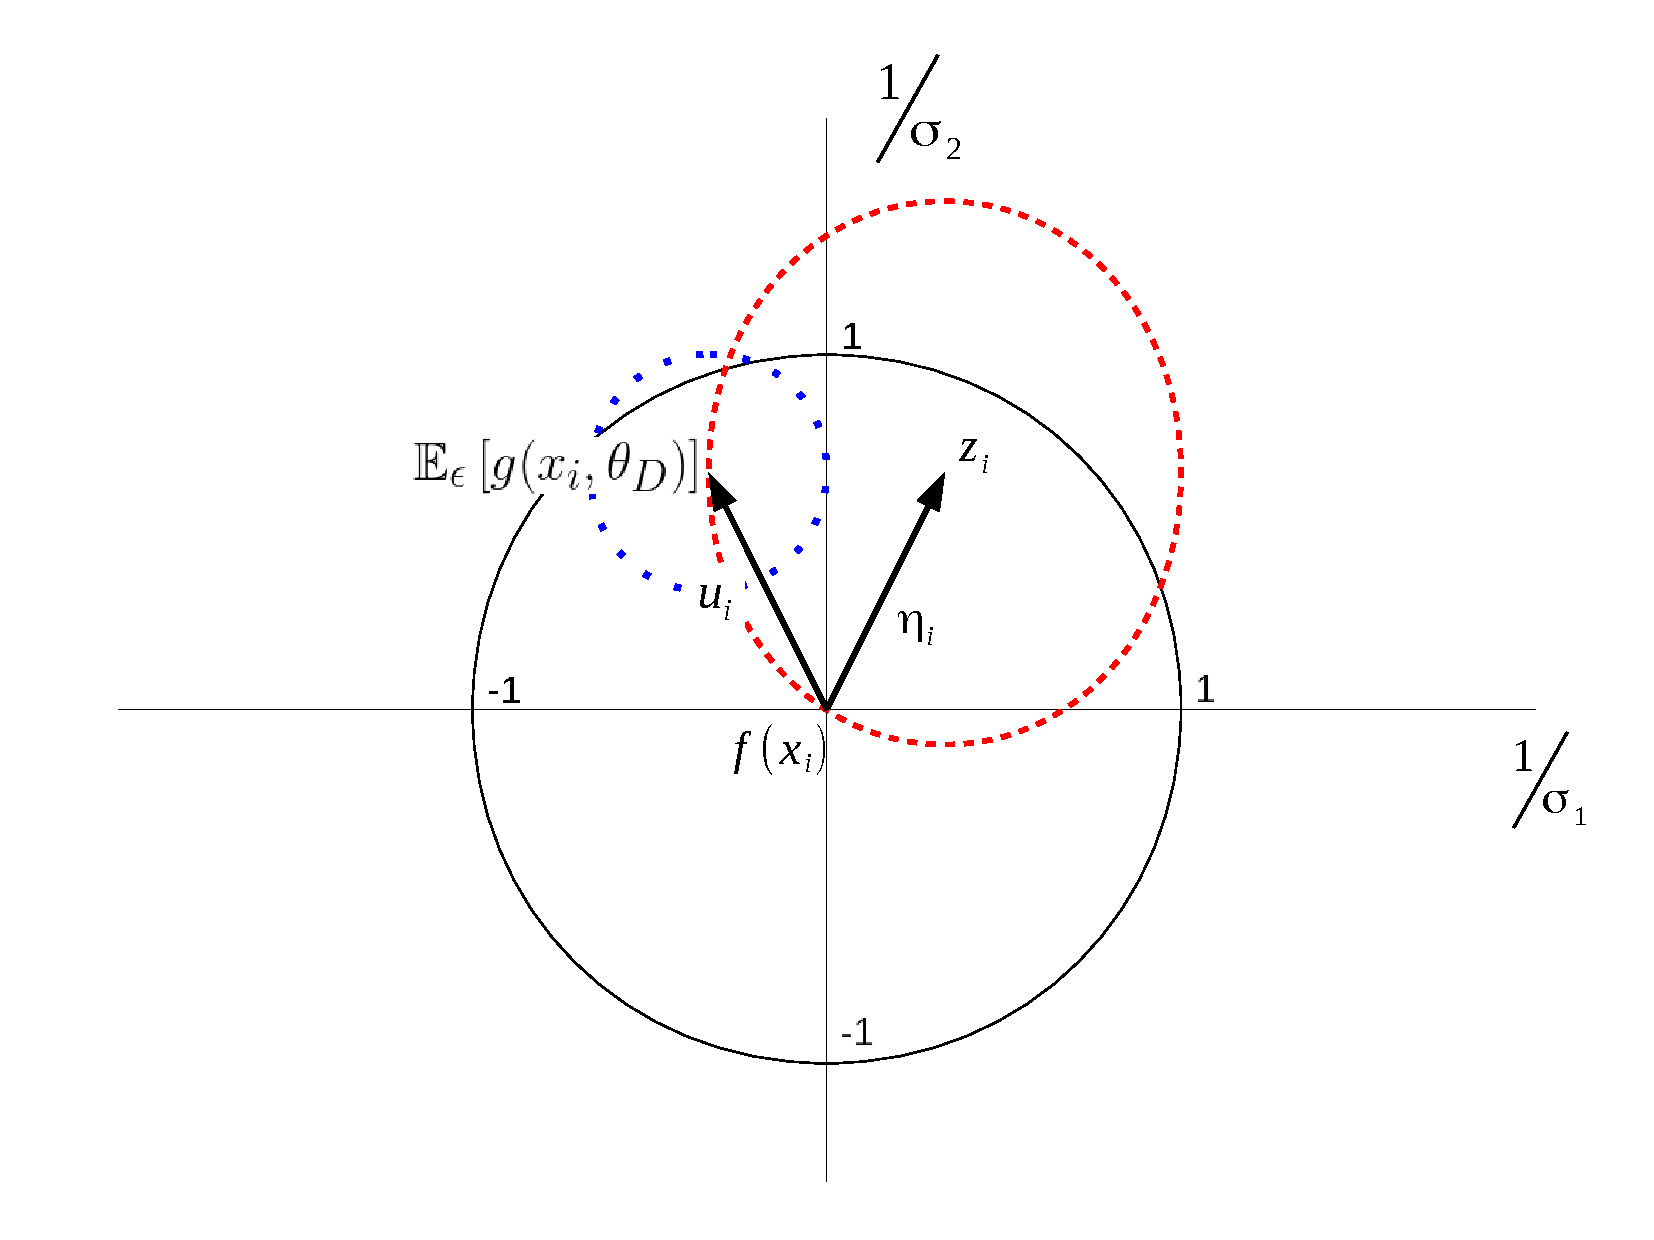
\includegraphics[width=\textwidth]{bias_variance_deltachi2_figure.pdf}
    \caption{example in 2D to visualise closure estimators, the axis
    is in units of $1/\sigma_{i}$ with $f(x_i)$ sitting at the origin.
    The black solid line is the $1 \sigma$ contour of the level 1 noise.
    $\dcs=0$ is represented by the red dashed
    ellipse, with $\dcs < 0$ and $\dcs > 0$ being inside and outside the ellipse
    respectively.\,{\em Bias} is $|u_i|^2$, {\em Noise} is $|\eta_i|^2$ and {\em Variance} is
    represented by the blue dashed line, as some ellipse centred on
    $\mathbb{E}_{\epsilon}\left[ g(x_i, \theta_D)\right]$. We see in this
    particular example that $\dcs=0$ however the expectation of the model does
    not reproduce the underlying law.}
    \label{fig:vectorexample}
\end{figure}
%

It is clear that the full story of whether a fit is better or not is given not
by a single estimator, but rather a combination of the estimators.

\subsubsection*{Summary}

\begin{itemize}
    \item Bias is the measure on whether we reproduce underlying law
    \item $\dcs$ gives an idea of where expected value of model is with relation
        to both underlying law and level 1 data
    \item All closure test estimators must be defined with same covariance matrix
        for a consistent picture, in the end this is what seperates sqrt(Variance) from $\phi$
        in the context of adding a theory uncertainty
    \item Whilst in fit to experimental data we don't have access to bias,
        figure \ref{fig:vectorexample} highlights that in a PDF fit we are not
        necessarily interested in the value of $\chis$ to the experimental data
        if we have high confidence that our model has low bias, which we can
        show with rigorous closure tests. Although low $\chis$ is probably
        preferred on a political level.
\end{itemize}
